\documentclass[a4paper]{article}

\usepackage{mathtools}
\usepackage{tikz}
\usetikzlibrary{automata,positioning,arrows,shapes,matrix}

\tikzset{
semithick,
node distance=1.5cm,
>=stealth,
initial text=,
every state/.style={draw,rectangle,rounded corners=2mm,inner sep=1mm,minimum height=2em},
accepting/.style={double distance=1pt,outer sep=0.9pt},
non/.style={draw,circle},
acc/.style={draw,circle,double,double distance=1pt,outer sep=0.9pt}
}


\begin{document}
\pagenumbering{gobble}

\begin{itemize} \itemsep3em
\item[] Automaton $\mathcal{A}$

\begin{tikzpicture}
\matrix[row sep=0.75cm,column sep=2cm]{
& \node[state,accepting] (1) {1}; & \node[state] (3) {3}; & \node[state] (6) {6}; & \\
\node[initial,state] (0) {0}; & & & \node[state,accepting](7) {7}; & \\
& & \node[state,accepting] (4) {4}; & & \node[state] (10) {$10$}; & \\
& \node[state] (2) {2}; & & \node[state] (8) {8}; & & \\
& & \node[state] (5) {5}; & \node[state] (9) {9}; & & \\
};

\path[->] (0) edge node[above] {$a$} (1)
              edge node[above] {$a$} (2)
          (1) edge node[above] {$a$} (3)
          (2) edge node[above] {$a$} (4)
              edge node[above] {$a$} (5)
          (3) edge node[above] {$a$} (6)
          (4) edge node[above] {$a$} (7)
              edge node[above] {$a$} (8)
          (5) edge node[above] {$a$} (9)
          (6) edge node[above] {$a$} (10)
          (7) edge node[above] {$a$} (10)
          (8) edge node[above] {$a$} (10)
          (9) edge node[above] {$a$} (10);
\draw[->] (10.south) .. controls +(-5cm,-10cm) and +(0cm,0cm) .. node[below] {$a$} (0.south);
\end{tikzpicture}

\vspace{-6cm}
\item[] Run tree of $\mathcal{A}$ on word $aaaa$ from state 0 to 10

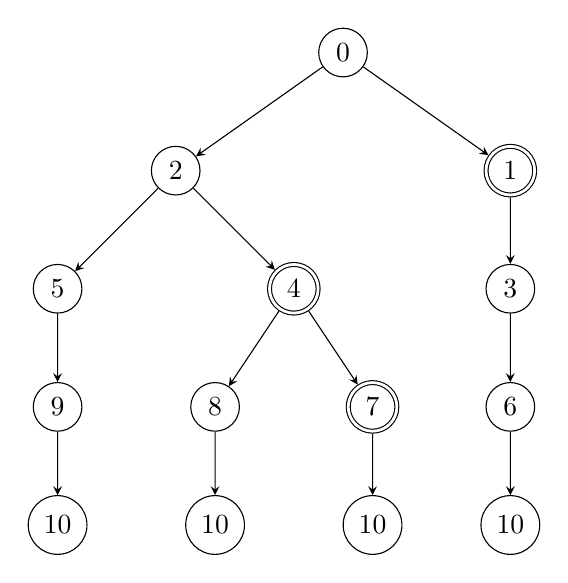
\begin{tikzpicture}[level 1/.style={sibling distance=4.25cm},
level 2/.style={sibling distance=3cm},level 3/.style={sibling distance=2cm},
level 4/.style={sibling distance=2cm},->]
\node[non] {0}
  child { node[non] {2}
    child {node[non] {5}
      child {node[non] {9}
        child {node[non] {10}}
      }
    }
    child {node[acc] {4}
      child {node[non] {8}
        child {node[non] {10}}
      }
      child {node[acc] {7}
        child {node[non] {10}}
      }
    }
  }
  child {node[acc] {1}
    child {node[non] {3}
      child {node[non] {6}
        child {node[non] {10}}
      }
    }
  };

% \node[initial,state] (0)                   {$\left(\{0\}\right)$};
% \node[state]         (01)   [right=of 0]   {$\left(\{0\},\{1\}\right)$};
% \node[state]         (012)  [right=of 01]  {$\left(\{0\},\{1\},\{2\}\right)$};
% \node[state]         (021)  [below=of 012] {$\left(\{0\},\{2\},\{1\}\right)$};

% \path[->] (0)   edge              node[above] {$a,b$} (01)
%           (01)  edge              node[above] {$a$}   (012)
%                 edge              node[above] {$b$}   (021)
%           (012) edge[loop above]  node        {$a,b$} ()
%           (021) edge              node[right] {$a$}   (012)
%                 edge[loop below]  node        {$b$}   ();
\end{tikzpicture}

\end{itemize}

\end{document}